Ein dreistöckiges Haus hat auf einer Seite $3\times 5$ ungefähr
gleich grosse Fenster, die über die Festtage mit verschiedenen Arten
von Lichterschmuck geschmückt werden sollen.
\begin{center}
\def\h{1.6}
\def\v{1.4}
\def\fenster#1#2{
\fill[color=blue!10] ({(#1-0.4)*\h},{(-0.7-(#2))*\v})
	rectangle ++({0.8*\h},{0.5*\v});
\draw ({(#1-0.4)*\h},{(-0.7-(#2))*\v}) rectangle ++({0.8*\h},{0.5*\v});
}
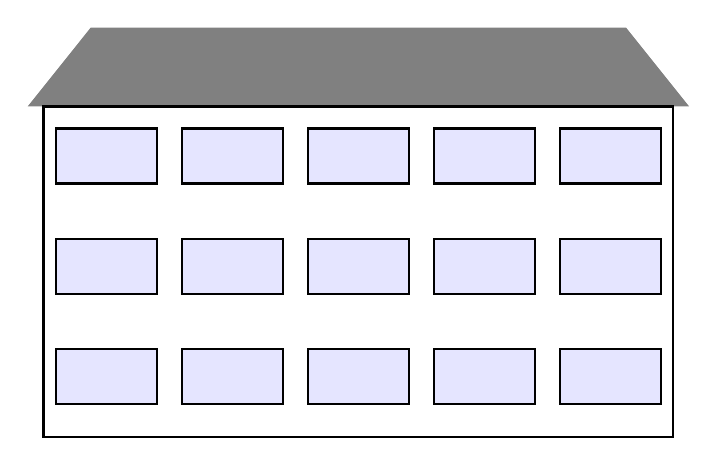
\begin{tikzpicture}[>=latex,thick]
\fill[color=gray] ({-2.5*\h-0.2},0) -- ({2.5*\h+0.2},0)
	-- ++(-0.8,1) -- ++({1.2-5*\h},0) -- cycle;
\draw ({-2.5*\h},{-3*\v}) rectangle ({2.5*\h},0);
\fenster{-2}{0}
\fenster{-1}{0}
\fenster{0}{0}
\fenster{1}{0}
\fenster{2}{0}
\fenster{-2}{1}
\fenster{-1}{1}
\fenster{0}{1}
\fenster{1}{1}
\fenster{2}{1}
\fenster{-2}{2}
\fenster{-1}{2}
\fenster{0}{2}
\fenster{1}{2}
\fenster{2}{2}
\end{tikzpicture}
\end{center}
\begin{teilaufgaben}
\item
Es stehen drei Arten von Dekorationen zur Verfügung, die jeweils
das Fenster vollständig ausfüllen: ein Stern,
ein Weihnachtsmann oder ein Engel.
Auf wieviele Arten können die Fenster dekoriert werden?
\item
Auf wieviele Arten können die Fenster mit 5 Weihnachtsmännern und 10 Sternen
dekoriert werden?
\item
Es sind bereits 6 Sterne, 5 Weihnachtsmänner und 4 Engel beschafft worden,
auf wieviele Arten können die Fenster damit dekoriert werden?
\item
Da das Gebäude spiegelsymmetrisch ist, sollen auch die Dekorationen
spiegelsymmetrisch angeordnet werden.
Auf wieviele Arten ist dies möglich?
(Die Einschränkungen der Teilaufgaben b) und c) gelten nicht mehr.)
\item
Auf wieviele Arten kann man die Fenster mit 7 Sternen, 5 Weihnachtsmännern
und 3 Engeln schmücken, wenn der Schmuck ausserdem spiegelsymmetrisch
sein soll.
\end{teilaufgaben}

\begin{loesung}
\begin{teilaufgaben}
\item
Dies ist ein Perlenkettenproblem, es können $3^{15}=14348907$ verschiedene
Dekarationen gewählt werden.
\item
Es sind die Plätze für die Weihnachtsmänner ausgewählt werden, dies ist auf
\[
\binom{15}{10}
=
\binom{15}{5}
=
\binom{15\cdot 14\cdot 13\cdot 12\cdot 11}{1\cdot 2 \cdot 3 \cdot 4 \cdot 5 }
=
7\cdot 13\cdot 3\cdot 11
=
3003
\]
Arten möglich.
\item
Zunächst sind die Plätze für die 6 Fenster für die Sterne gewählt werden,
dann unter den verbleibenden 9 Fenstern die 5 Fenster für die Weihnachtsmänner:
\begin{align*}
\binom{15}{6}\cdot\binom{9}{5}
&=
5005\cdot 126
=
630630
\intertext{oder mit Fakultäten geschrieben}
&=
\frac{15!\cdot 9!}{6!\cdot 9!\cdot 5!\cdot 4!}
=
\frac{15!}{6!\cdot 5!\cdot 4!}
=
630630.
\end{align*}
\item
Durch die Symmetrie sind Dekorationen in der rechten Hälfte des
Gebäudes bereits festgelegt, wenn die Dekorationen für die linke
Hälfte des Gebäudes ausgewählt wurden.
Es sind also 9 Dekoration zu wählen, was auf $3^9=19683$ Arten möglich ist.
\item
Die Symmetrie bedeutet, dass je ein Stern, ein Weihnachtsmann und ein
Engel für die mittleren Fenster gewählt werden müssen.
Dies ist ein Reihenfolgeproblem für 3 Objekte, welches auf $3!=6$ Arten
gelöst werden kann.
Die verbleibenden Dekorationen müssen symmetrisch verteilt werden, als
gleich viele auf jeder Seite.
Es reicht daher zu zählen, auf wieviele Arten 3 Sterne, 2 Weihnachtsmänner
und 1 Engel auf 6 Fenster verteilt werden können.
Dies ist auf
\begin{align*}
\binom{6}{3}\cdot\binom{3}{2}
&=
20\cdot 3
=
60
\\
&=
\frac{6!}{3!\cdot 3!}\cdot\frac{3!}{2!\cdot 1!}
=
\frac{6!}{3!\cdot 2!}
=
\frac{6!}{6\cdot 2}=\frac{5!}2=\frac{120}2 = 60
\end{align*}
Arten möglich.
Insgesamt gibt es also $3!\cdot 60 = 360$ Möglichkeiten.
\qedhere
\end{teilaufgaben}
\end{loesung}

\begin{bewertung}
Symmetrieüberlegung in Teilaufgabe e) ({\bf S}) 1 Punkt,
Jede Teilaufgabe ({\bf A} -- {\bf E}) 1 Punkt.
\end{bewertung}


